\documentclass[11pt,a4paper]{article}
\usepackage[utf8]{inputenc}
\usepackage[german]{babel}
\usepackage[T1]{fontenc}
\usepackage{amsmath}
\usepackage{amsfonts}
\usepackage{amssymb}
\usepackage{graphicx}
\usepackage[margin=1.25cm]{geometry} % Puts the same margin on all borders of the document

% Packages

\usepackage{hyperref} % Generate hyperlinks to referenced items
\usepackage{adjustbox} % Used to change parameters in \includegraphics[scale=•]{•}
\usepackage{enumitem} % Provides several options for lists
\usepackage{verbatim} % Package to use \begin{comment}
\usepackage{pdfpages} % Used to import PDF pages
\usepackage{multirow} % Allows us to have a single cell in a table span multiple rows
\usepackage{makecell} % Allows us to format multiple lines in a single cell
\usepackage{listings} % Used to type code in \begin{lstlisting}
\usepackage{xcolor}  % Gives access to coloring text
\usepackage{longtable} % Allows us to create a table over multiple pages
\usepackage{float} % Improved placement of floating items
\usepackage{pdfpages} % Used to import pdf pages
\usepackage{booktabs} % Used for horizontal lines instead of \hline



% Settings

\graphicspath{{./files/}} % Sets path for files to the files folder in the same directory

\hypersetup{
    colorlinks=false, %set true if you want colored links
    linktoc=all,     %set to all if you want both sections and subsections linked
    linkcolor=blue,  %choose some color if you want links to stand out
}


\begin{titlepage}
  \title{AUD Reference Sheet} % document_name-type_of_document
  \author{Frederick Wichert}
  \date{Last Edited: \today}
\end{titlepage}


\begin{document}
	\pagenumbering{gobble}
	\maketitle
	
	\setcounter{secnumdepth}{2}
	\setcounter{tocdepth}{2}
	\tableofcontents
	
	\newpage
	\pagenumbering{arabic}




\section{Begriffsdefinitonen}%% 								Definitionen 
	\paragraph{Problem}
	Ein Problem im Sinner der Informatik enthält eine Beschreibung der Eingabe, der Ausgabe, aber keinen Übergang. \\
	Eine \textbf{Probleminstanz} eine bestimmte Belegung der Eingabevariablen

	\paragraph{Algorithmus}
	Ein Algorithmus ist eine endliche Folge von Rechenschritten, die eine Eingabe in eine Ausgabe umwandelt.

	\paragraph{Datenstruktur}
	Eine Datenstruktur ist eine Methode, Daten abzuspeichern und zu organisieren, sowie deren Zugriff auf die Daten und die Modifikation der Daten zu erleichtern.



\vspace{1.5cm}
\section{Pseudocode} %% 			 							Pseudocode
	\subsection{Aufbau}
	\begin{itemize}
		\item Pseudocode folgt keinen festen Regeln und dient der Veranschaulichung.
		\item Er entspricht Code einer beliebigen Programmierspracheund folgt keiner Sprachspetifischen Syntax, ist aber an solche angelehnt. 
		\item Keywords werden in Caps geschrieben 
	\end{itemize} 

	\subsection{Beispiele}
	\subsubsection{Initiliasieiren von Variablen}
	\texttt{variable = value;}

	\subsubsection{Schleifen und Anweisungen}
	\texttt{WHILE bedingung ...} \\
	\hspace{0.4cm} \texttt{ENDWHILE} \\ \\
	\texttt{FOR value TO value} \\
	\texttt{IF bedingung THEN vlaue} \\

	\subsubsection{Arrays}
	- Üblicherweise als \texttt{A} bezeichnet \\
	\texttt{A[i] = ... ;}



\vspace{1.5cm}
\section{Algorithmen} %% 										Algorithmen

\subsection{Definition}
	Ein Algorithmus ist eine endliche Folge von Rechenschritten, die eine Eingabe in eine Ausgabe umwandelt.

	\subsection{Anforderungen}
	$\rightarrow$ Spezifizirung der Eingabe und Ausgabe \\
	$\rightarrow$ Eindeutigkeit - Jeder Einzelschritt ist klar definiert mit festgelgeter Reihenfolge \\
	$\rightarrow$ Endlichkeit - Die Notation hat eine Endliche Länge

	\subsection{Eigenschaften}
	$\rightarrow$ Determiniertheit - Für gleiche Eingabe wird gleiche Ausgabe berechnet (mögliche, andere Zwischenzustände) \\
	$\rightarrow$ Determinismus - Für die gleiche Eingabe ist die Ausführung und Ausgabe identisch \\
	$\rightarrow$ Terminierung - Der Algorithmus läuft für jede Eingabe nur endlich lange \\
	$\rightarrow$ Korrektheit - Der Algorithmus berechnet stets die spezifizierte Ausgabe, falls dieser terminiert \\
	$\rightarrow$ Effzienz - Sparsamkeit bei Ressourcen (Zeit, Speicher, Energie etc.)



\vspace{1.5cm}
\section{Effizienz von Algorithmen} %% 							Effizienz von Algorithmen

	\begin{itemize}
		\item Effizienzfaktoren
		\begin{itemize}
			\item Rechenzeit (Anzahl der Einzelschritte)
			\item Kommunikationsaufwand (z.B. Netzwerk)
			\item Speciherplatzbedarf 
			\item Zugriff auf Speicher (z.B. Festplatte) \\
		\end{itemize}
		\item  (Konkret) Laufzeit hängt von vielen Faktoren ab
		\begin{itemize}
			\item Länge der Eingabe 
			\item Implementierung der Basisoperationen
			\item Takt der CPU
		\end{itemize}
	\end{itemize}



\vspace{1.5cm}
\section{Asymptotische Komplexität} %% 							Asymptotische Komplexität
	Eine Abschätzung des (zetilichen) Aufwands eines Algorithmus in Abhängigkeit der Eingabe
	in form einer Asymptote in Abhängigkeit der Eingabemenge $n$.

	\begin{itemize}
		\item Beispiel: Summe bis n
		\begin{itemize}
			\item \texttt{summe=summe+i}
			\item Ablauf:
			\begin{itemize}
				\item Variablen deklarieren
				\item 1 zur Summe addieren
				\item 2 zur Summer addieren
				\item \dots
				\item n zur Sumer addieren
				\item Ausgabe der Summe
			\end{itemize}
			\item Alle Basisoperationen benötigen konstant viel Aufwand 
			\item Anzahle der Operationen wächst mit Eingabe n
			\item Für liner wachsende Eingabe wächst der Aufwand auch linear
		\end{itemize}
		\item Beispiel: Laufzeit von InsertionSort
		\begin{itemize}
			\item Quadratische Funktion: $an^2 + bn + c$
			\item Bei gro\ss em n überweigt der quadratische Anteil $\rightarrow$ Terme niedriger Ordnung werden irrelevant
			\item s
		\end{itemize}
	\end{itemize}


	\subsection{Asymptotische Notation}
	\begin{itemize}
		\item Wie ist das Verhalten der Laufzeit $T(n)$ für sehr gro\ss e Eingaben $  \in N$
		\begin{itemize}
			\item bei kleinen Eingaben (z.B. $n = 5$) ist die reale Laufzeit mehr dominiert 
				von den Initialisierungskosten und nicht dem Algorithmus selbst
			\item Komplexität ist unabhängig von konstanten Faktoren und Summanden
			\item Berücksichtigen nicht Betrachtung:
			\begin{itemize}
				\item Rechnergeschwindigkeit
				\item Aufwände der Initialisierung
			\end{itemize}
			\item Komplexitätsmessungen via Funktionsklassen ausreichend
			\begin{itemize}
				\item Wie verhält sich der Algorithmus für gro\ss e Problemgrö\ss en
				\item Wie verändert sich die Laufzeit, wenn die Problemgrö\ss e verdoppelt wird
			\end{itemize}
		\end{itemize}
	\end{itemize}

	\paragraph{Komplexitätsfunktion} \mbox{} \\
	Das Wachstumsverhalten reicht aus um die wichtigen Punkte eines Algorithmus zu veranschaulichen.

	\subsection{Schranken der asymptotischen Komplexität}
	\paragraph{Best case}
	\begin{itemize}
		\item Komplexität im "besten" Fall
		\item Wie schnell ist der Algorithmus, wenn der Input so vorliegt, dass dieser am schnellsten terminiert?
		\item Beispiel: Vorsortierte Liste für (simplen) Sortieralgorithmus
	\end{itemize}
	\paragraph{Average case}
	\begin{itemize}
		\item Komplexität im "durchschnittlichen" Fall
		\item Wie schnell ist der Algorithmus, wenn ein üblicher Input vorliegt?
		\item Beispiel: Zufällig verteilte Liste für (simplen) Sortieralgorithmus
	\end{itemize}
	\paragraph{Worst case}
	\begin{itemize}
		\item Komplexität im "schlechtesten" Fall
		\item Wie schnell ist der Algorithmus, wenn der Input so vorliegt, dass dieser am spätestens terminiert?
		\item Beispiel: Negativ-sortierte Liste für (simplen) Sortieralgorithmus
	\end{itemize}

	\subsection{Notationen und Definition}
	\paragraph{$\Theta$-Notation}
	\begin{center}
		Funktion en $f, g: \mathbb{N} \rightarrow \mathbb{R}_{>0}$ \\
	\end{center}
	Dabei ist $\mathbb{N}$ Die Eingabelänge und $\mathbb{R}$ die Zeit 
	\begin{center}
		$\Theta(g) = \{f: \exists c_1 , c_2 \in \mathbb{R}_{>0}, n_0 , \in \mathbb{N}, \forall n \geq n_0 , 0 \leq c_1 g(n) \leq f(n) \leq c_2 g(n)\}$
	\end{center}
	Schreibweise: $f \in \Theta (g)$ oder $f = \Theta (g)$

	\paragraph{O-Notation}
	Obere asymptotische Schranke
	\begin{center}
		$O(g) = \{f: \exists c \in \mathbb{R}_{>0}, n_0 , \in \mathbb{N}, \forall n \geq n_0 , 0 \leq f(n) \leq c g(n)\}$
	\end{center}
	Sprechweise: $f$ wächst höchstens so schnell wie g \\
	Sprechewise: $f = O(G)$ \\\\

	\noindent Beachte: $f(n) = \Theta (n) \implies f(n) = O(n)$ \\
	\indent \hspace{1.5cm} $\Theta (g(n)) \subseteq O(g(n))$ \\

	\noindent Rechenregeln
	\begin{itemize}
		\item Konstanten: $f(n) = a$ mit $a \in \mathbb{R}$ konstante Funktion. Dann $f(n) = O(1)$
		\item Skalare Multiplikation: $f = O(g)$ und $a \in \mathbb{R}$. Dann $a*f = O(g)$
		\item Addition: $f_1 = O(g_1)$ und $f_2 = O(g_2)$. dann $f_1 + f_2 = O(max\{ g_1, g_2\})$
		\item Multiplikation: $f_1 = O(g_1)$ und $f_2 = O(g_2)$. dann $f_1 * f_2 = O(g_1 * g_2)$
	\end{itemize}

	\paragraph{$\Omega$-Notation}
	Untere asymptotische Schranke
	\begin{center}
		$\Omega(g) = \{f: \exists c \in \mathbb{R}_{>0}, n_0 , \in \mathbb{N}, \forall n \geq n_0 , 0 \leq c g(n) \leq f(n)\}$
	\end{center}
	Sprechweise: $f$ wächst mindestens so schnell wie g \\
	Sprechewise: $f = \Omega(G)$ \\

	\begin{center}
		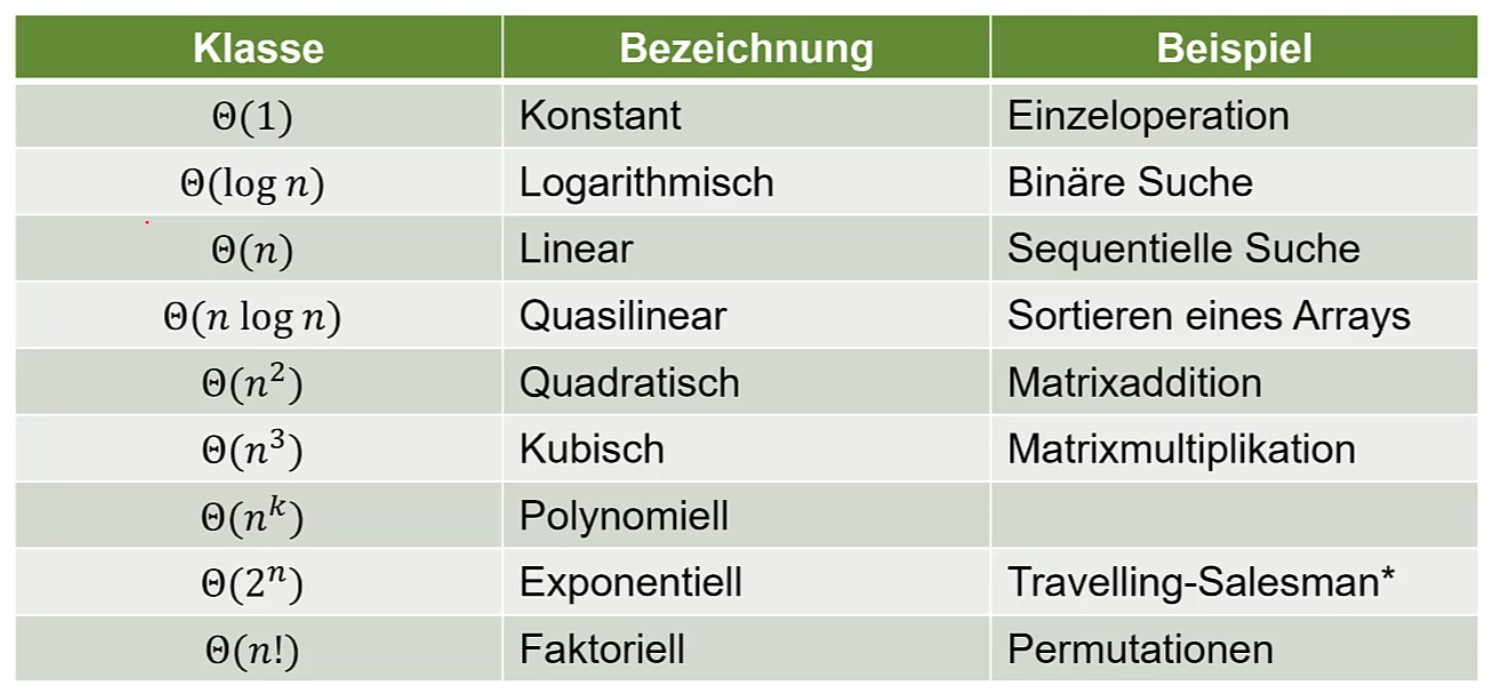
\includegraphics[scale=0.4]{Notation_Exsample.jpg}
	\end{center}



\vspace{1.5cm}
\section{Analyse von Divide-and-Conquer Algorithmen} %% 		D-a-C Analyse

	$T(n)$ ist Laufzeit eines Problems der Grö\ss e $n$. \\ \\
	\noindent Für kleines Problem, d.h. $n \leq c$ mit $c$ ist eine Konstante, dann benötigt 
	die Direkte Lösung konstante Zeit $\Theta (1)$. \\ \\
	\noindent Für sonstige $n$ gilt: Das Aufteilen des Problems führt zu $a$ Teilproblemen, 
	von denen jedes die grö\ss e 1/$b$ der Grö\ss e des ursprünglichen Problems hat. \\ \\
	\noindent Das Lösen eines Teilproblems der Grö\ss e $n$/$b$ dauert $T(n/b)$ und somit 
	benötigen wir für das Lösen von $a$ solcher Probleme $aT(n/b)$. \\ \\
	\noindent $D(n)$ ist die Zeit um das Problem aufzuteilen, $C(n)$ ist die Zeit um die 
	Teillösungen zur Lösung des ursprünglichen Problems zusammenzufügen. \\

	\begin{center}
		\[
			T(n) = \left\{\begin{array}{lr}
				\Theta (1) & \\
				aT(n/b) + D(n) + C(n) &
				\end{array}\right\}
		\] \\
		Falls $n \leq c$ \vspace{1cm}
	\end{center}


	\paragraph{Methoden zur Lösung von Rekursionsgleichung} \mbox{} \\

	\noindent \textbf{Substitutionsmethode:} wir erraten eine Schranke und nutzen methematische Induktion, 
	um die Korrektheit zu beweisen.

	\noindent \textbf{Rekursionsbaum-Methode:} wandelt die Rekursionsgleichung in einen Baum um, 
	dessen Knoten die Kosten der Rekursion in den versxchiedenen Ebenen darstellt.

	\noindent \textbf{Mastermethode:} leifert Schranken für Rekursionsgleichung der Form: $T(n) = aT(n/b) + f(n)$


	\paragraph{Substitutionsmethode}
	Zur Lösung der Rekursionsgleichung, 2 Schritte:
	\begin{itemize}
		\item Rate die Form der Lösung, z.B. durch 
		\begin{itemize}
			\item Scharfes Hinsehen
			\item kurze Eingaben ausprobieren und einsetzen
		\end{itemize}
		\item Anwendung von vollständiger Induktion, um die Konstante zu finden und zu zeigen, dass
			das Geratene eien Lösung ist
	\end{itemize}


	\paragraph{Rekursionsbaum-Methode}
	Grundidee: Stelle das Ineinander-Einsetzen als Baum dar und analysiere die Kosten
	\begin{enumerate}
		\item Jeder Knoten stellt die Kosten eines Teilproblems dar.
		\begin{itemize}
			\item Die Wurzel stellt die zu analysierenden Kosten $T(n)$ dar
			\item Die Blätter stellen die Kosten der Basisfälle dar, z.B. $T(0)$
		\end{itemize}
		\item Berechnen die Kosten innerhalb jeder Ebene des Baums
		\item Die Gesamtkosten ist die Summe über die Kosten aller Ebenen
	\end{enumerate}
	Geratenes kann durch Substitutionsmethode überprüft werden.


	\paragraph{Mastermethode}
	Allgemeine Form der Rekursionsgleichung: \\
	\noindent $T(n) = aT(n/b) + f(n)$ mit $q \geq 1, b > 1$ und $f(n)$ eine asymptotische positive Funktion.

	\begin{itemize}
		\item Problem wird in $a$ Teilprobleme der grö\ss e $n/b$ aufgeteilt.
		\item Lösen jedes der $a$ Teilprobleme benötigt Zeit $T(n/b)$.
		\item Funktion $f(n)$ umfasst die Kosten, um das Problem in Teilprobleme aufzuteilen
			und um die Teillösungen zu vereinigen.
	\end{itemize}

	\paragraph{Mastertheorem}
	Seien $a \geq 1$ und $b > 1$ Konstanten. Sei $f(n)$ eine positive Funktion und $T(n)$
	über den nicht negativen ganzen Zahlen durch die Rekursionsgleichung
	\begin{center}
		$T(n) = aT(n/b) + f(n)$
	\end{center}
	definiert, wobei wir $n/b$ so interpretieren, dass damit entweder $\lfloor n / b \rfloor$
	oder $\lceil n/b \rceil$ gemeint ist. Dann besitzt $T(n)$ die folgenden asymptotischen Schranken:
	\begin{enumerate}
		\item Gilt $f(n) = O(n^{\log_b a-\epsilon})$ für eine Konstante $\epsilon > 0$, dann $T(n) = \Theta (n^{\log_b a})$.
		\item Gilt $f(n) = \Theta (n^{\log_b a})$, dann gilt $T(n) = \Theta (n^{\log_b a} \lg n)$.
		\item Gilt $f(n) = \Omega (n^{\log_b a+\epsilon})$ für eine Konstante $\epsilon > 0$ und $af(n/b) \leq cf(n)$
			für eine Konstante $c < 1$ und hinreichend gro\ss en $n$, dann ist $T(n) = \Theta (f(n))$.
	\end{enumerate} 
	Das Mastertheorem verstehen: \\
	In jedem der 3 Fälle wird die Funktion $f(n)$ mit $n^{\log_b a}$ verglichen. \\
	Intuition:  
	\begin{enumerate}
		\item Wenn $f(n)$ olynomial kleiner ist als $n^{\log_b a}$, dann $T(n) = \Theta (n^{\log_b a})$.
		\item Wenn $f(n)$ und $n^{\log_b a}$ die gleiche Gr\ss e haben, dann gilt $T(n) = \Theta (n^{\log_b a} \lg n)$.
		\item Wenn $f(n)$ polinimial gr\ss er ist als $n^{\log_b a}$ und $af(n/b) \leq cf(n)$ erfüllt, dann ist $T(n) = \Theta (f(n))$.
	\end{enumerate}
	\textbf{Nicht} abedeckte Fälle sind:
	\begin{enumerate}
		\item Wenn $f(n)$ kleiner als $n^{\log_b a}$, aber nicht polinimial klainer.
		\item Wenn $f(n)$ grö\ss er als $n^{\log_b a}$, aber nicht polinimial grö\ss er.
		\item Regularitätsbedingung $af(n/b) \leq cf(n)$ nicht erfüllt.
	\end{enumerate}




\vspace{1.5cm}
\section{Datenstrukturen: Theorie} %% 									Datenstrukturen

	\subsection{Besipiele}
	\begin{center}
		\begin{tabular}{ p{4cm} | p{4cm} | p{4cm} }
			\makecell[c] {\textbf{Grundlegende} \\ \textbf{Datenstrukturen}} &
			\makecell[c] {\textbf{Fortgeschrittene} \\ \textbf{Datenstrukturen}} &
			\makecell[c] {\textbf{Randomisierte} \\ \textbf{Datenstrukturen}} \\

			\makecell[c] {Stacks} &
			\makecell[c] {Rot-Schwarz-Bäume} &
			\makecell[c] {Skip Lists} \\
			
			\makecell[c] {Verkettete Listen} &
			\makecell[c] {AVL-Bäume} &
			\makecell[c] {Hash Tables} \\

			\makecell[c] {Queues} &
			\makecell[c] {Splay-Bäume} &
			\makecell[c] {Bloom-Filter} \\

			\makecell[c] {Bäume} &
			\makecell[c] {Heaps} &
			\makecell[c] {} \\

			\makecell[c] {Binäre Suchbäume} &
			\makecell[c] {B-Bäume} &
			\makecell[c] {} \\
		\end{tabular}
	\end{center}
	\vspace{1cm}

	\paragraph{Begriffsunterscheidung} \mbox{} \\
	Abstrakter Datentyp ("was") \\
	Beschreibt Stack mit Operationen \\
	Datenstrukturen ("wie") \\
	Beschreibt die Stack-Operationen als Array oder Verkettete Liste




\vspace{1.5cm}
\section{Datenstruktur: Stacks}

	\paragraph{Operationen:}
	\begin{itemize}
		\item new(S)		- erzeugt neuen (leeren) Stack
		\item isEmpty(S)	- gibt an, ob Stack S leer ist
		\item pop(S)		- gibt oberstes Element vom Stack S zurück und löscht es, falls vorhanden
		\item push(S,k)		- schreibt k als neues oberstes Element auf S
		\item $\longrightarrow$ LIFO - last in, first out
	\end{itemize}
	\begin{center}
		Intuitive erwartete Bedingugen sind erfüllt, auch ohne algebraische Spezifikiation
	\end{center}

	\paragraph{Darstellung als Array} \mbox{} \\
	\begin{center}
		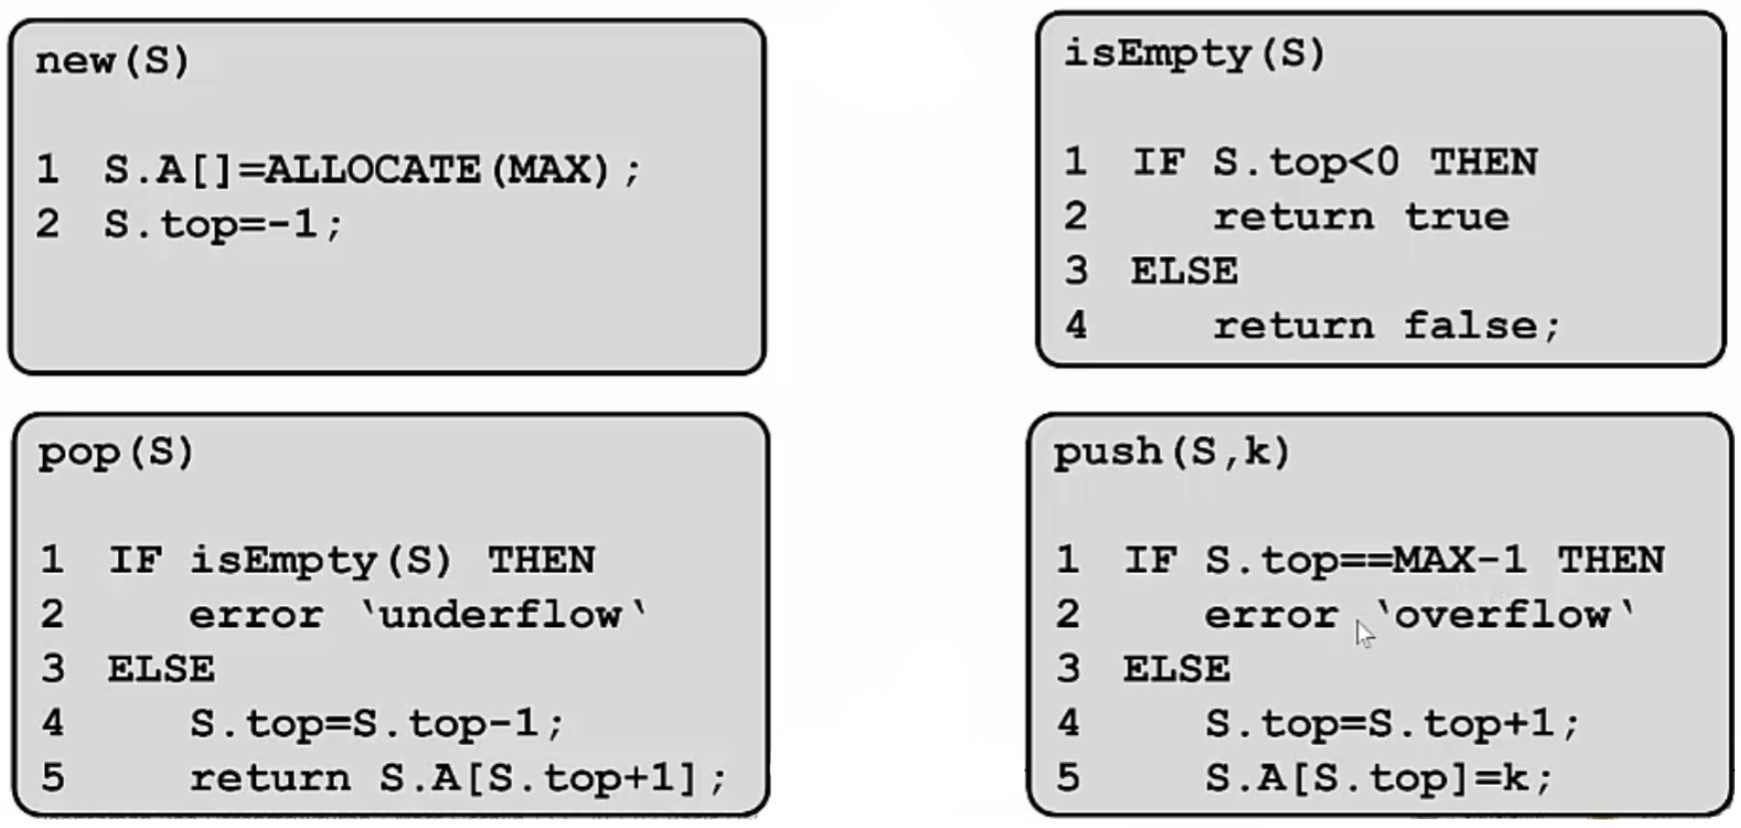
\includegraphics[scale=0.4]{Stack_Operationen_Code.jpg}
	\end{center}

	Bei der Darstellung als Array kann die maximale Grö\ss e erreicht werden. Danach wird beim 
	Hinzufügen das ganze Array in ein größeres kopiert. Da dies in $\Theta (n^2)$ liegt wird ein
	Faktor festgelegt. So wird beispielweise bei erreichen der maximalen Grö\ss e die Grö\ss e
	verdoppelt, haben wir weniger als 1/Faktor*Faktor, also weniger als ein Viertel der Elemente belegt
	so halbieren wir unser Array.




\vspace{1.5cm}
\section{Datenstruktur: Verkettete Listen}

	\begin{center}
		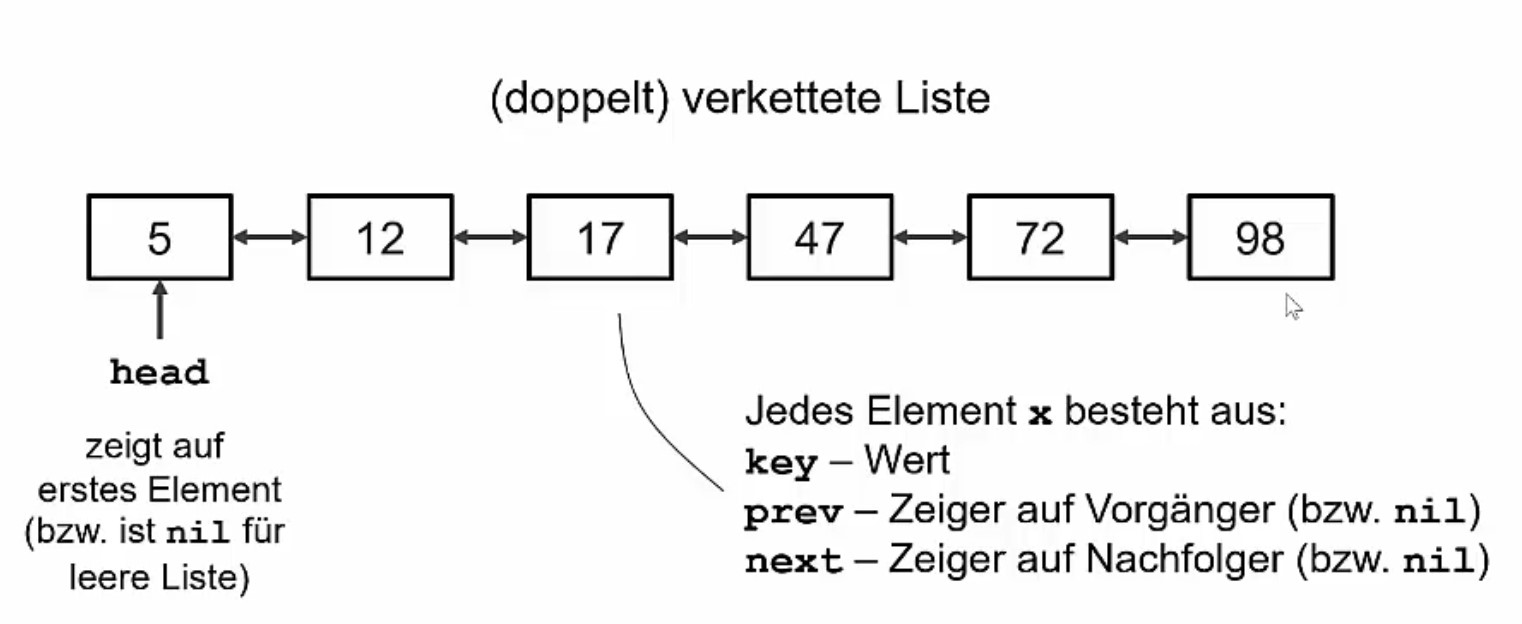
\includegraphics[scale=0.4]{Doppelt_Verkettete_Listen_Bsp.jpg}
	\end{center}

	

\section{Datenstruktur: Queues}

	Operationen:
	\begin{itemize}
		\item new(Q) - erzeugt neue (leere) Queue
		\item isEmpty(Q) - gibt an, ob Queue leer ist
		\item dequeue(Q) - gibt vorderstes Element der Queue zurück und löscht es
		\item enqueue(Q,k) - schreibt k als neuees hinterstes Element auf Q
		\item $\longrightarrow$ FIFO - first in, first out
	\end{itemize}

	\paragraph{Darstellung als Array} \mbox{} \\
	Bei der Darstellung als Array stö\ss t man nun auf Probleme. Es werden nun zwei Zeiger, 
	und nicht mehr wie bei Stacks nur einer, benötigt. Da die Schlange aber nun durch das 
	Array durchwandert bleibt sehr viel Arrrayplatz ungenutzt, bzw. man bräuchte ein unendlich
	gro\ss es Array. Daher gibt es zwei Darstellungsmöglichkeiten:
	\begin{center}
		Als Array: \hspace{5cm} Als zyklisches Array:\\
		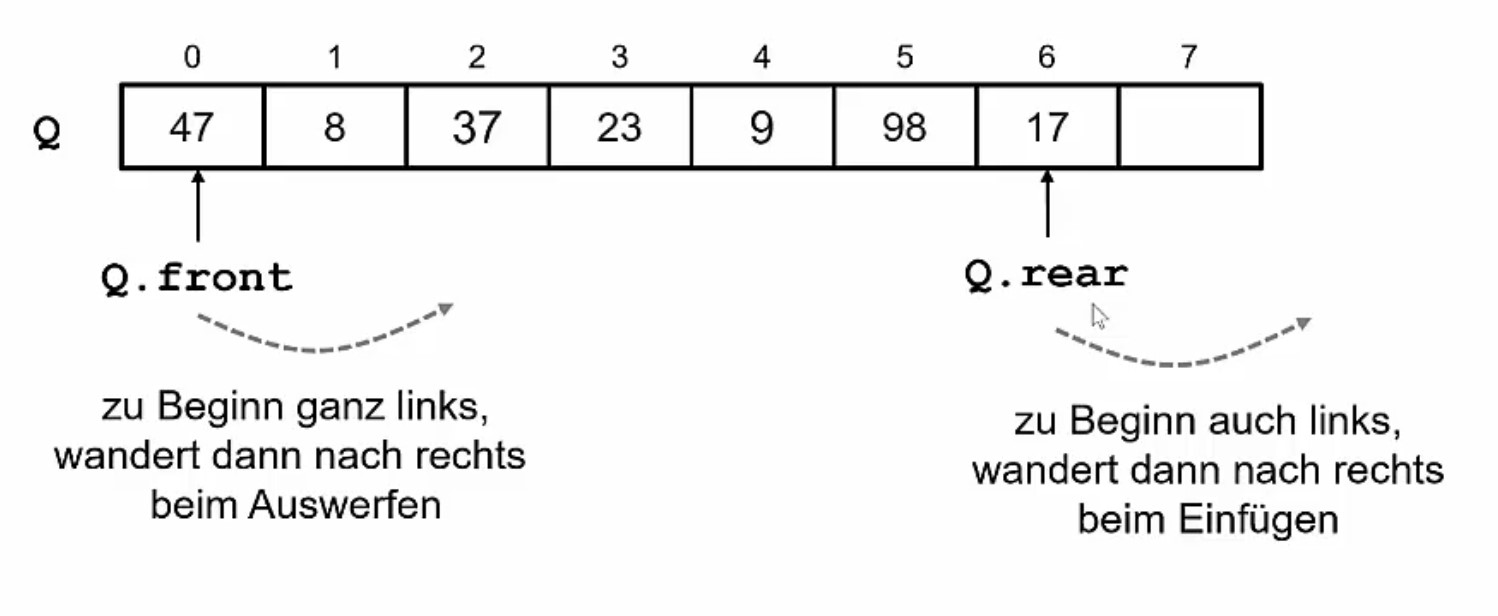
\includegraphics[scale=0.3]{Queues_Array.jpg}
		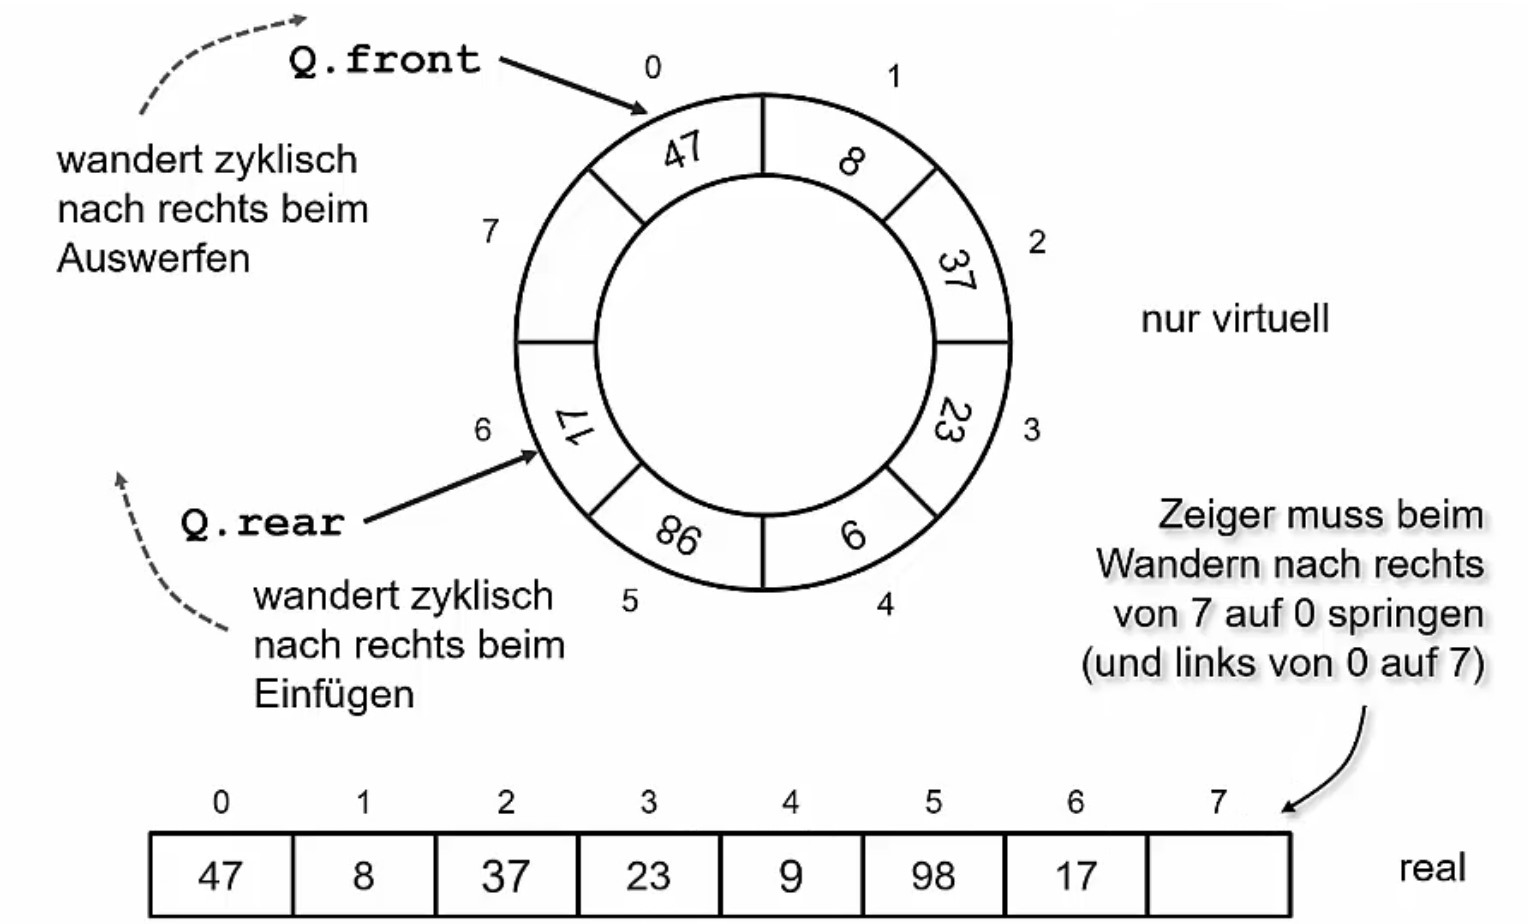
\includegraphics[scale=0.3]{Queues_Array_Zyklisch.jpg}
	\end{center}





\vspace{1.5cm}
\section{Datenstruktur: Binärbüume}

	Operationen:
	\begin{itemize}
		\item new(Q)
	\end{itemize}

	\paragraph{Darstellung als Array} \mbox{} \\
	Bei der Darstellung als A
	\begin{center}
		Als Array: \hspace{5cm} Als zyklisches Array:\\
		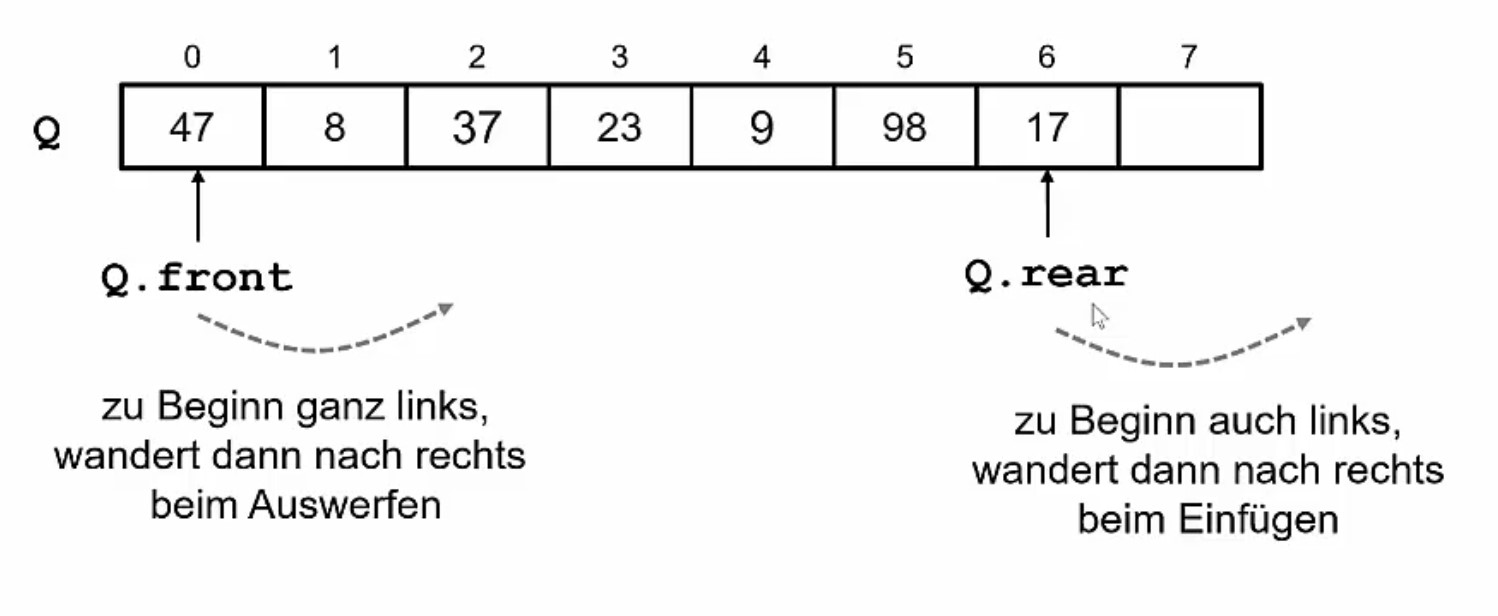
\includegraphics[scale=0.3]{Queues_Array.jpg}
		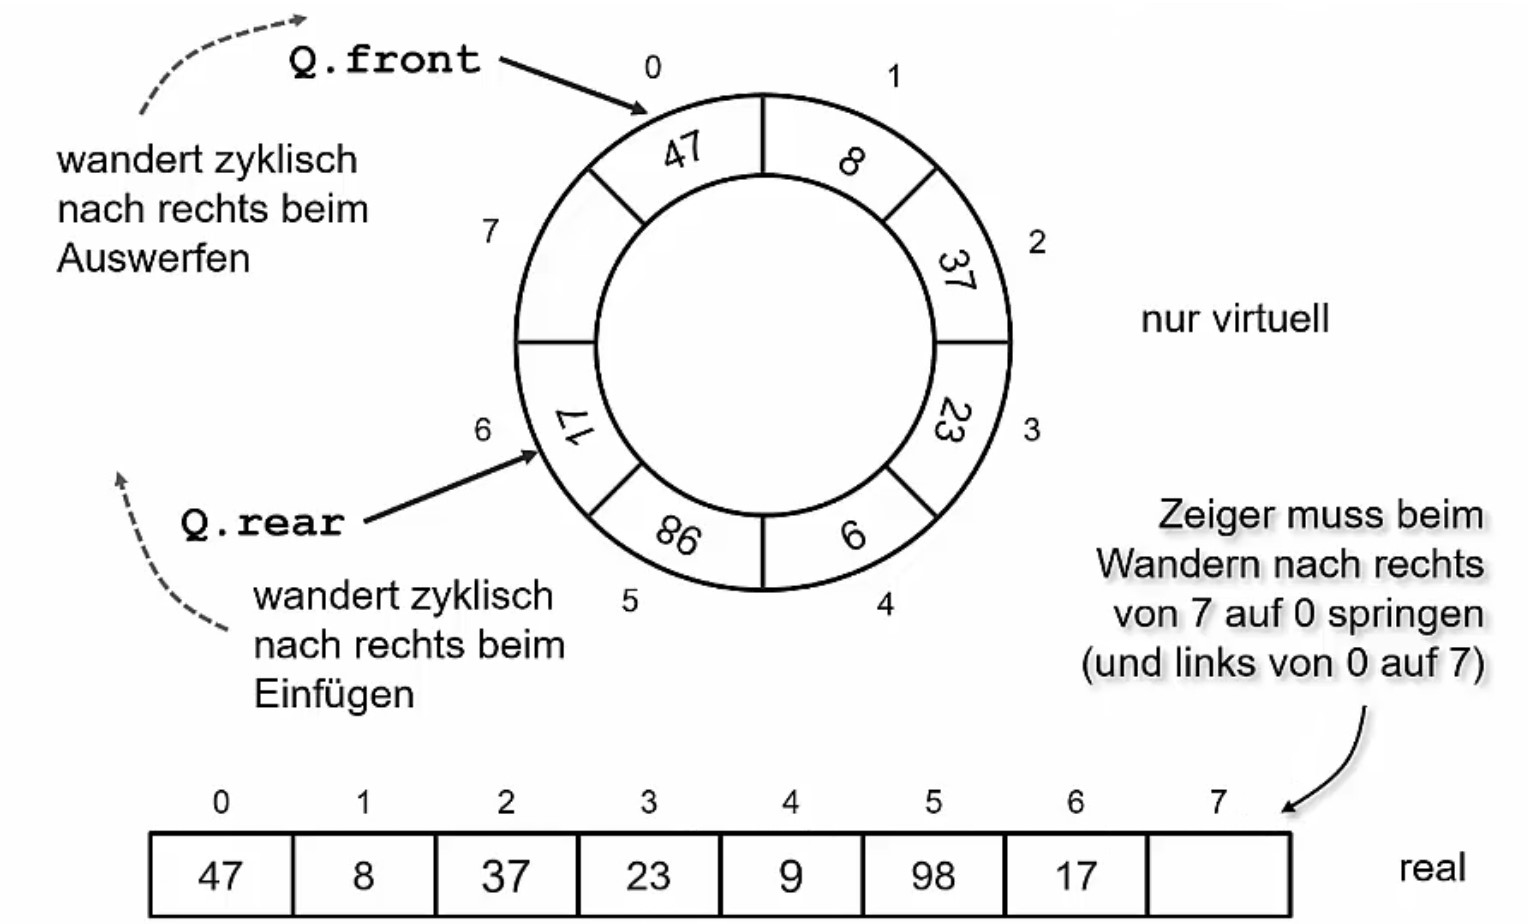
\includegraphics[scale=0.3]{Queues_Array_Zyklisch.jpg}
	\end{center}





\vspace{1.5cm}
\section{Sortieralgorithmen: Theorie} %% 								Sortieralgorithme

	\subsection{Warum möchte man Sortieren}
	\begin{itemize}
		\item Sachen Packen
		\item Zeitmanagement
		\item etc
	\end{itemize}

	\subsection{Bedingungen}
	- Ausgangspunkt als Folge von Datensätzen \\
	- Zu sortierenden elemente hei\ss en Schlüsselelemente (-werte) \\
	- Ziel: Schlüsselwerte nach einem Ordnungsschlüssel zu sortieren \\
	\textbf{Bedingug} $\rightarrow$ Schlüsselwerte müssen vergleichbar sein

	\subsection{Vergleichskriterien}
	- Berechnungsaufwand: O(n) \\
	- Effizienz: Best Case vs. Average Case vs. Worst Case \\ 
	- Speicherbedarf:
	$\rightarrow$ in-place: zustzlicher Speicher von der Eingabegrö\ss e unabhängig \\
	$\rightarrow$ out-of-place: Speichermerhbedarf von eingabegrö\ss e abhängig \\
	- Stabilität: Erahltenbleiben des sekundären Sortierschlüssels \\

	$\rhd$ Sortierverfahren abhängig von Anwendung, Unterschiedliche Zahl von Vertauschungen vs Vergleichungen 

	\subsection{Vergleichsverfahren}

	\subsubsection{Korrektheit mittels Schleifeninvariante}
	\begin{itemize}
		\item Eine Schleifeninvariante beschreibt was bei dem Durchlauf einer Schleife zu Beginn immer gegeben ist \\
			Damit kann die Korrektheit eines Algorithmus bewiesen werden \\
			$\rhd$ Vergleichbar mit einem Indutkionsbeweis 
		\item Eine Schleifeninvariante muss 3 Eigenschaften erfüllen:
		\begin{itemize}
			\item Initialisierung: Invariante ist vor jeder Iteration wahr
			\item Fortsetzung: Wenn die Invariante vor der Schleife wahr ist dann bleibt sie auch bis zum Beginn der nächsten Iteration wahr
		\end{itemize}
		\item Bei dem Insertionsort:
		\begin{itemize}
			\item Zu Beginn ist die Leinke Teilmenge immer sortiert
		\end{itemize}
	\end{itemize}



\vspace{1.5cm}
\section{Entwurfsprinzipien des Sortieren} %% 					Entwurfsprinzipien des Sortieren

	$\rhd$ IsertionSort: inkrementelle Herangehenweise \\ \\

	\noindent $\rhd$ Divide-and-Conquer Ansatz (Teile-undBeherrsche):
	\begin{itemize}
		\item Ansatz um Sortieralgorithmus zu entwerfen
		\item Laufzeit: im schlechtesten Fall immer noch besser als InsertionSort
		\item Gibt Methoden mit welchen wir die Laufzeit einfach bestimmen können \\
	\end{itemize}

	\subsection{Devide-and-Conquer}
	\paragraph{Prinzip:} Zerlege das Problem und löse es direkt \textit{oder} durch weitere Zerlegung.
	\paragraph{Divide:} Teile das Problem in mehrere Teilprobleme auf, die kleinere Instanzen des gleichen Problems darstellen.
	\paragraph{Conquer:} Beherrsche die Teilprobleme rekursiv. Wenn die Teilprobleme klein genug sind, dann löse die Teilprobleme auf direktem Weg.
	\paragraph{Combine:} Vereinige die Lösung der Teilprobleme zur Lösung des ursprünglichen Problems.

	\begin{center}
		Beispiel: \underline{\nameref{MergeSort}}
	\end{center}


\vspace{1.5cm}
\section{Sortieralgorithmus: InsertionSort} %% 					Beispiele: Insertionsort 


\paragraph{Grundidee}
	\begin{itemize}
		\item Sortieren durch Einfügen:
		\item Die Linke Teilmenge ist Sortiert, und passend wird immer ein neues Element eingefügt 
	\end{itemize}

	\paragraph{Eigenschaften}
	\begin{itemize}
		\item Stabieler Algorithmus
	\end{itemize}

	\paragraph{Code}
	\begin{center}
		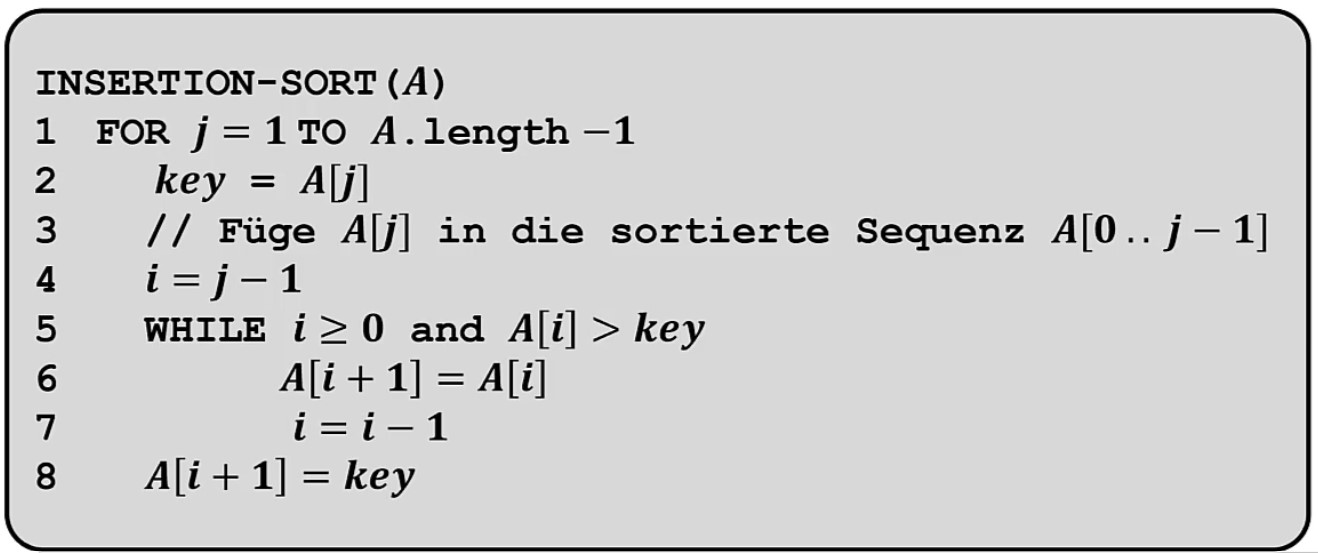
\includegraphics[scale=0.45]{InsertionSort_Code.jpg}
	\end{center}

	\paragraph{Beweis der Korrektheit} \mbox{} \\
	Um die Korrekthiet des Algorithmuses zu bestimmen nutzen wir die Schleifeninvariante
	\begin{itemize}
		\item Initialisierung: Beginn mit j=1, also mit dem Teilfeld bis j-1, besteht aus einem element und ist Sortiert
		\item Fortsetzung: Zu zeigen ist, dass die Invariante bei jeder Iteration erhalten bleibt.
			Die for-Schleife verschiebt jedes Element der sortierten Menge um eins nach rechts bis das zu
			sortierende Element eingefügt werden kann. Inkrementieren von j erhält die Schleifeninvariante
		\item Terminierung: Abbruhcbedingung for-Schleife wenn j>A.length-1. Jede Itearation erhöht j.
			Dann bei Abbruch j=n und einsetzen in Invariante liefert das Teilfeld A[0...n-1] welches aus den
			ursprünglichen Elementen besteht $\rightarrow$ Teilfeld = gesamtes Feld
	\end{itemize}



\vspace{1.5cm}
\section{Sortieralgorithmus: BubbleSort} %% 					Beispiele: BubbleSort

\paragraph{Grundidee} \mbox{} \\
$\rhd$ Vergleiche Paare von benachbarten Schlüsselwerten \\
$\rhd$ Tausche das Paar, falls rechter Schlüsselwert kleiner ist als linker

\paragraph{Code} \mbox{} \\
\begin{center}
	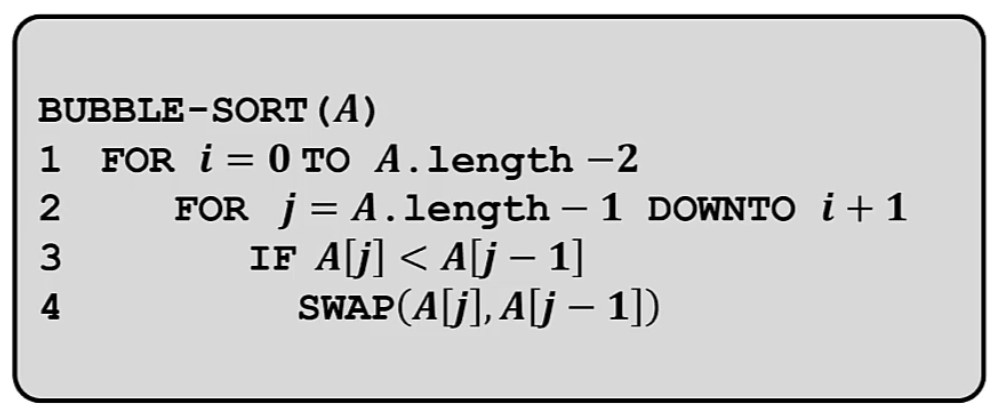
\includegraphics[scale=0.5]{BubbleSort_Code.jpg}
\end{center}

\paragraph{Analyse} \mbox{} \\
Anzahl der Vergleiche
\begin{itemize}
	\item es werden stets alle Elemente er Teilfolge verglichen
	\item unabhängig von der Sortierung
\end{itemize}
Anzahl der Vertauschungen
\begin{itemize}
	\item Best case: 0 Vertauschungen
	\item Worst case: $\frac{n^2 - n}{2}$ Vertauschungen
\end{itemize}
Komplexität
\begin{itemize}
	\item Best case: $\Theta (n)$
	\item Average case: $\Theta (n^2)$
	\item Worst case: $\Theta (n^2)$
\end{itemize}



\vspace{1.5cm}
\section{Sortieralgorithmus: SelectionSort} %% 					Beispiele: SelectionSort

	\paragraph{Grundidee} \mbox{} \\
	$\rhd$ Sortieren durch direktes Auswählen
	\begin{itemize}
		\item MinSort: "wähle kleinstes Element in Array und tausche es nach vorne
		\item MaxSort: "wähle grö\ss etes Element in Array und tausche es nach hinten
	\end{itemize}

	\paragraph{Code} \mbox{} \\

	\begin{center}
		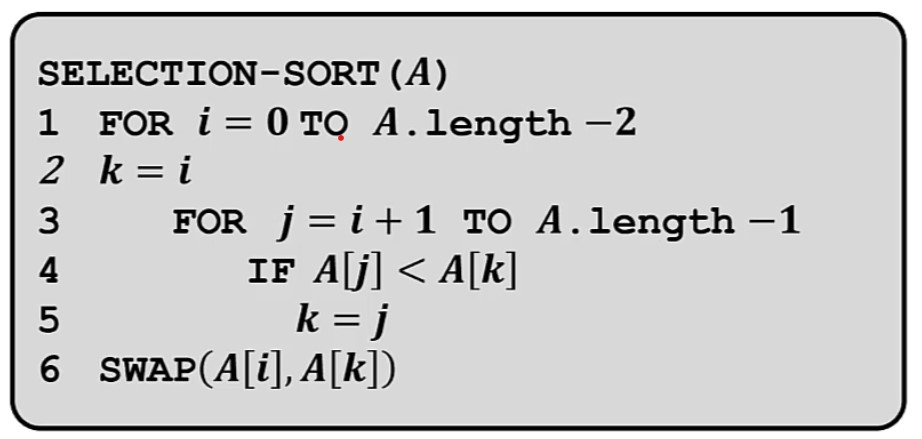
\includegraphics[scale=0.5]{SelectionSort_Code.jpg}
	\end{center}



\vspace{1.5cm}
\section{Sortieralgorithmus: MergeSort} %% 						Beispiele: SelectionSort
	\label{MergeSort}

	\paragraph{Grundidee} \mbox{} \\
	$\rhd$ Baut auf dem Devide-and-Conquer Prinziep auf
	\begin{itemize}
		\item \textbf{Divide:} Teile die Folge mit $n$ Elementen in zwei Teilfolgen von je $\frac{n}{2}$ Elementen auf
		\item \textbf{Conquer:} Sortiere die zwei Teilfolgen rekursiv mithilfe von MergeSort
		\item Vereinige die zwei sortierten Teilfolgen, um die sortierte Lösung zu erzeugen
	\end{itemize}


	\paragraph{Code} \mbox{} \\

	\begin{center}
		Prinziep des MergeSorts \\
		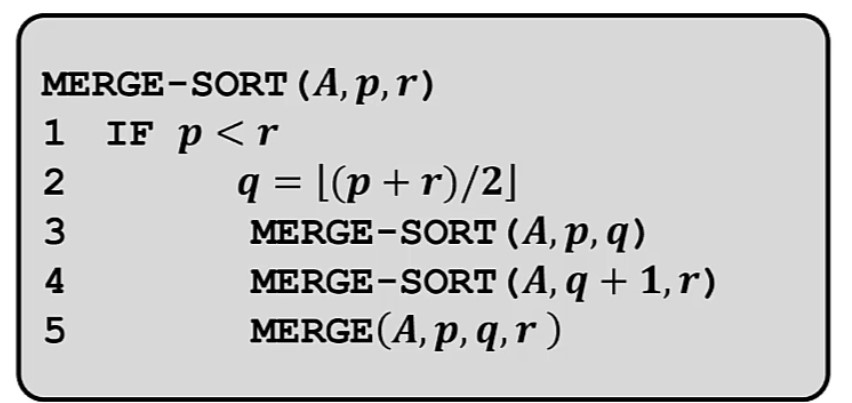
\includegraphics[scale=0.53]{MergeSort_Code.jpg}
	\end{center}
	\mbox{} \\
	Beim Halbieren wird immer abgerundet, so kann jede Teilfolge sortiert werden. \\ \\

	\begin{center}
		Prinziep des gesamtes Codes \\
		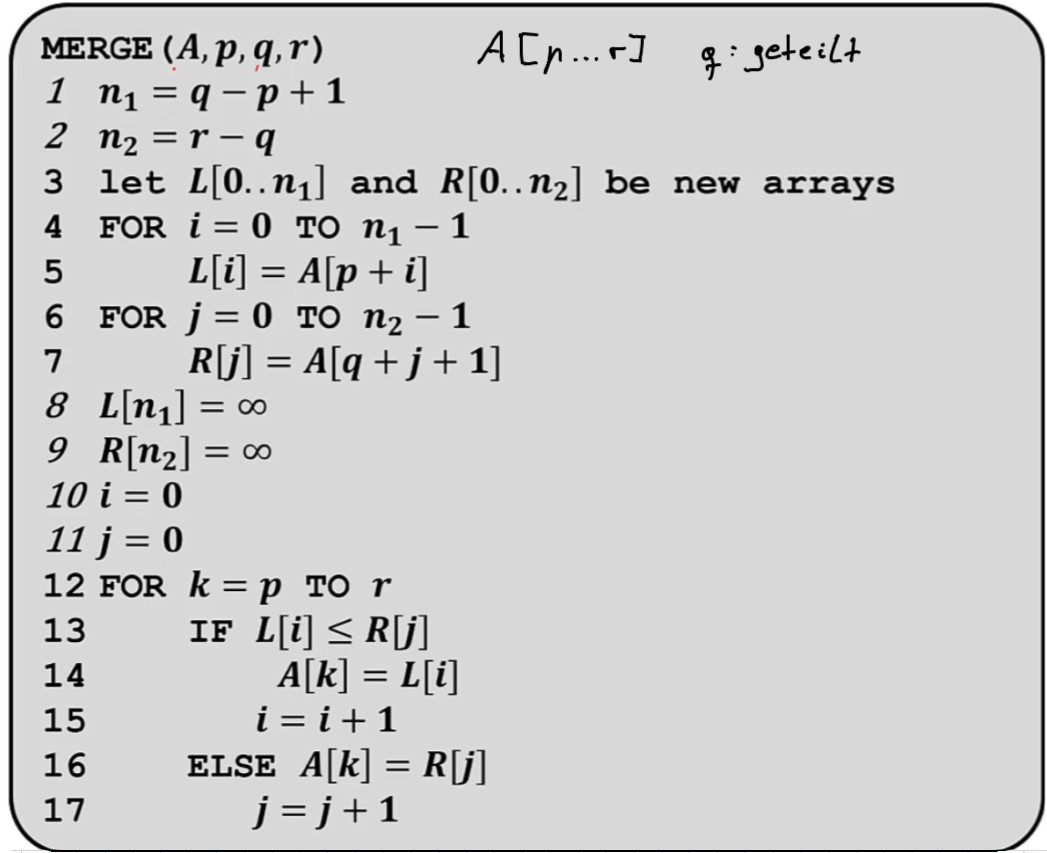
\includegraphics[scale=0.5]{MergeSort_Komplett_Code.jpg}
	\end{center}
	\mbox{} \\ \\


	\paragraph{Analyse} \mbox{} \\
	\textbf{Ziel:} Bestimme Rekursionsgleichung für Laufzeit $T(n)$ von $n$ Zahlen im schlechtesten Fall
	\begin{itemize}
		\item \textbf{Divide:} Es wird einfach die Mitte des Feldes berechnet. Dies benötigt konstante Zeit, also $\Theta(1)$
		\item \textbf{Conquer:} Wir lösen zwei Teilprobleme der Grö\ss e $\frac{n}{2}$ rekursiv. Dies trägt mit $2T(\frac{n}{2})$ uir Laufzeit bei
		\item \textbf{Combine:} Die Prozedur \texttt{MERGE} auf einem Teilfeld der Länge $n$ lineare Zeit, also $\Theta(n)$
	\end{itemize}

	\begin{center}
		\[
			T(n) = \left\{\begin{array}{lr}
				c & \text{falls } n = 1 \\
				2T(\frac{n}{2}) & \text{falls } n > 1 
				\end{array}\right\}
		\] \vspace{0.35cm}

		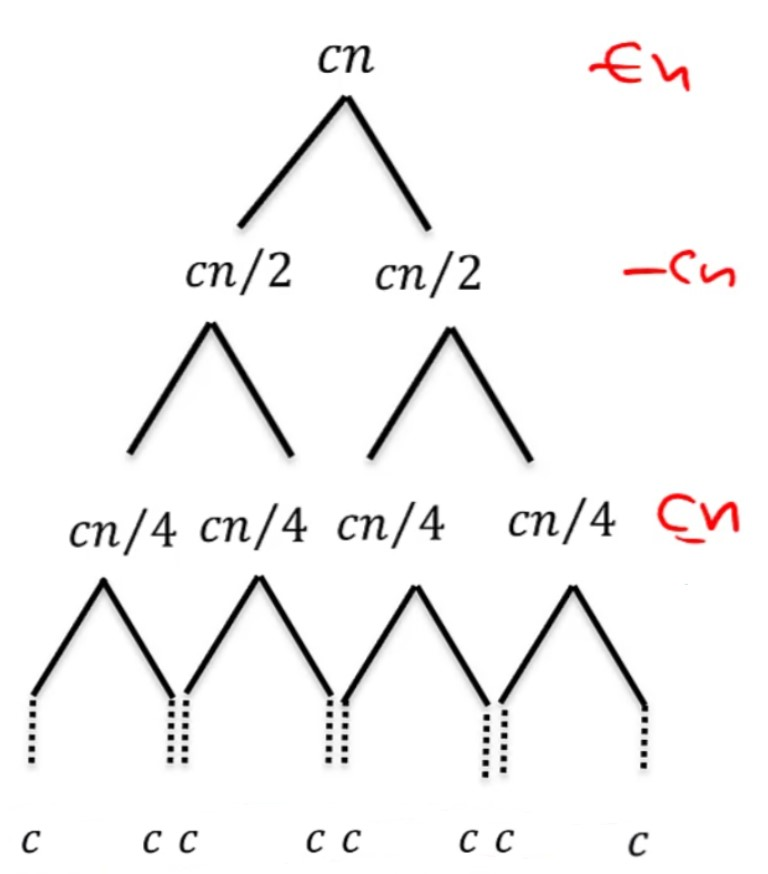
\includegraphics[scale=0.35]{MergeSort_BinaryTree.jpg}
	\end{center}

	Daraus ergibt sich eine Komplexität von $\Theta(n \log n)$ \\



	\paragraph{Beweis der Korrektheit} \mbox{} \\
	\textbf{Schleifeninvariante:} Zu Beginn jeder Iteration der for-Schleife (Zeile 12-17) enthält 
	das Teilfeld $A[p...k-1]$ die $k-p$ kleinsten Elemente aus $L[0...n_1]$ und $R[0...n_2]$ 
	in sortierter Reihenfolge. Weiter sind $L[i]$ und $R[j]$ die kleinsten Elemente ihrer 
	Arrays, die noch nicht zurück kopiert wurden. \\
	\textbf{Initialisierung:} Vor der ersten Iteration gilt $k = p$. \\ Daher ist $A[p...k-1]$
	leer und enthält $0$ kleinste Elemente von $L$ und $R$. Wegen $i = j = 0$ sind $L[i]$ und
	$R[j]$ die kleinsten Elemente ihrer Arrays, die noch nicht zurück kopiert wurde. \\
	\textbf{Fortsetzung:} Müssen zeigen, dass Schleifeninvariante erhalten bleibt. Dafür nehmen wir an,
	dass $L[i] \leq R[j]$. Dann ist $L[i]$ kleinstes Element, welches noch nicht zurück kopiret wurde.
	Da Array $A[p...k-1]$ die $k - p$ kleinsten Elemente enthält, wird der Array $A[p...k]$ die 
	$k - p + 1$ kleinsten Elemente enthalten nachdem der Wert nach der Durchführung von Zeile 14 
	kopiert wurde. Nach Erhöung der Variablen $k$ und $i$ stellt die Schleifeninvariante für die 
	nächste Iteration wieder her. \\ Wenn $L[i] > R[j]$ dann analoges Argument mit Zeilen 16-17.
	\textbf{Terminierung:} Beim Abbruch gilt $k = r + 1$. Durch die Schleifeninvariante enthält 
	$A[p...r]$ die kleinsten Elemente von $L[0...n_1]$ und $R[0...n_2]$ in sortierter Reihenfolge.
	Alle Elemente au\ss er der Sentinels wurden korrekt zurück kopiert.



\vspace{1.5cm}
\section{Sortieralgorithmus: QuickSort} %% 						Beispiele: QuickSort

	\paragraph{Grundidee}
	\begin{itemize}
		\item Wähle ein Pivotelement $x$ des Arrays
		\item Zerlege den Array in zwei Teilarrays
		\begin{itemize}
			\item Erster Teilarray: Enthält alle Elemente $y \leq x$
			\item Zweiter Teilarray: Enthält alle Elemente $y > x$ 
		\end{itemize}
		\item Sortiere rekursiv auf den Teillisten mit Quicksort
		\item Einelementige Listen sin schon sortiert
	\end{itemize}

	Dies lässt sich auf das Prinziep von Divide-and-Conquer zurückführen:

	\begin{itemize}
		\item \textbf{Divide:} Zerlege das Array $A[p...r]$ in zwei Teilarrays $A[p...q-1]$ 
			und $A[q+1...r]$, sodass jedes Element aus $A[p...q-1]$ kleiner oder gleich $A[q]$
			ist, welches wiederum kleiner oder gleich jedem Element von $A[q+1...r]$ ist. 
			Berechnen den Index $q$ als Teil vom Partition Algorithmus.
		\item \textbf{Conquer:} Sortieren beider Teilarrays $A[p...q-1]$ und $A[q+1...r]$ durch
			rekursiven Aufruf von Quicksort
		\item \textbf{Combine:} Da die Teilarrays bereits sortiert sind, ist keine weitere Arbeit
			nötig um diese zu vereinigen. $A[p...r]$ ist nun sortiert. 
	\end{itemize}



	\paragraph{Code} \mbox{} \\

	\begin{center}
		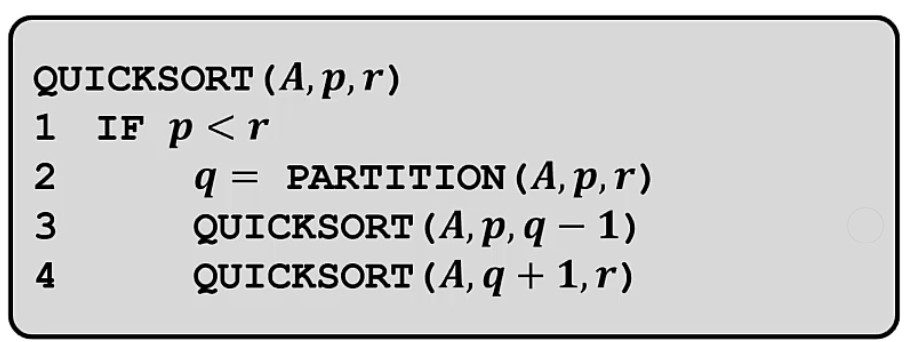
\includegraphics[scale=0.5]{QuickSort_Code_Partition.jpg} \\ \vspace{0.5cm}
		Im Folgenden gucken wir uns den Algorithmus genauer an: \\ \vspace{0.5cm}
		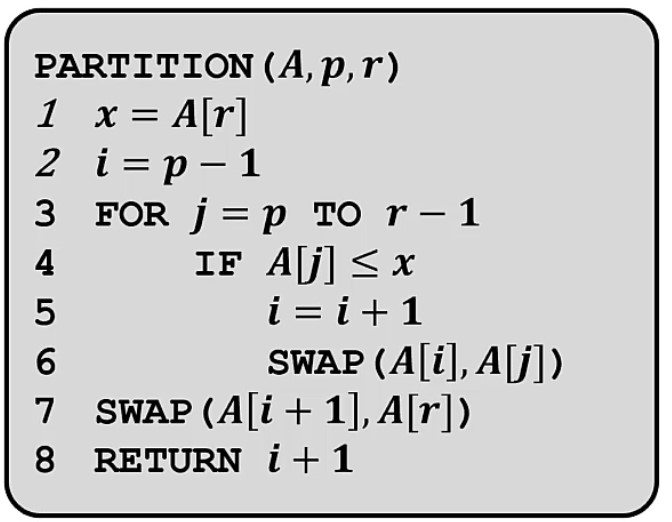
\includegraphics[scale=0.5]{QuickSort_Code.jpg} \\ \vspace{0.5cm}
		Zeile 1: Pivotelement wählen \\
		Zeile 2: Index $i$ setzen \\
		Zeile 3-6: Teilarrays mit Element füllen \\
		Zeile 7: Pivotelement tauschen \\
		Zeile 8: Neuer Index des Pivotelements \\ \vspace{0.9cm}
		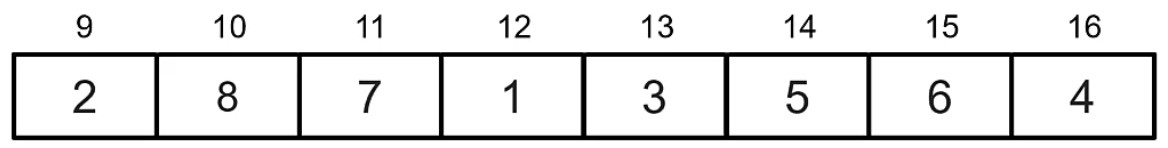
\includegraphics[scale=0.4]{QuickSort_Code_PartitionSample_01.jpg} \\
		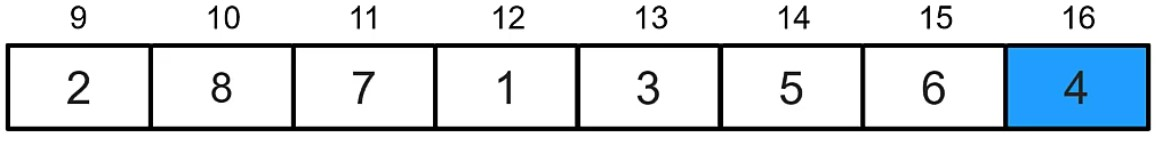
\includegraphics[scale=0.4]{QuickSort_Code_PartitionSample_02.jpg} \\
		. \\
		. \\
		. \\
		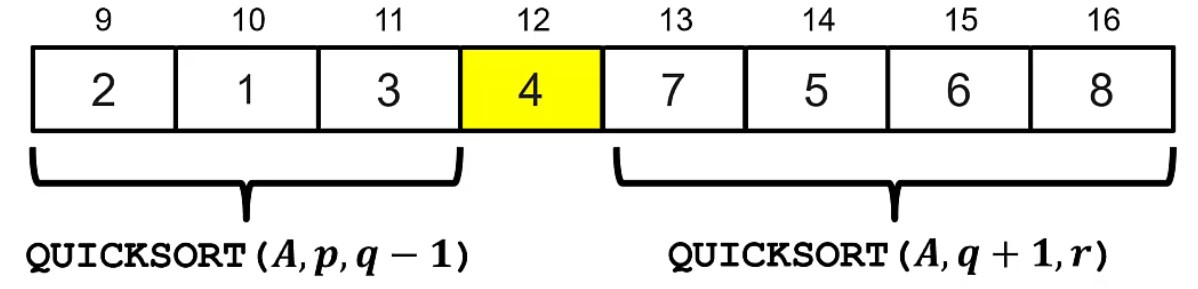
\includegraphics[scale=0.4]{QuickSort_Code_PartitionSample_00.jpg} \\
	\end{center}



	\paragraph{Korrektheit von Quicksort} \mbox{} \\
	\begin{itemize}
		\item \textbf{Schleifeninvariante:} Zu Beginn jeder Iteration der for-Schleife (Zeile3-6)
			gilt für den Arrayindex $k$ folgendes:
		\begin{itemize}
			\item Ist $p \leq k \leq i$, so gilt $A[k] \leq x$.
			\item Ist $i + 1 \leq k \leq j - 1$, so gilt $A[k] > x$.
			\item Ist $k = r $, so gilt $A[k] = x$.
		\end{itemize}
		\item \textbf{Initialisierung:} Vor der ersten Iteration gilt $i = p-1$ und $j = p$.
			Da es keine Werte zwischen $p$ und $j$ gibt und es auch keine Werte zwischen $i+1$ 
			und $j-1$ gibt, sind die ersten beiden Eigenschaften trivial erfüllt. \\
			Die Zuweisung in Zeile 1 sorgt für die Erfüllung der dritten Eigenschaft.
		\item \textbf{Fortsetzung:} Zwei mögliche Fälle durch Zeile 4. \\
			Wenn $A[j] > x$, dann inkrementiert die Schleife ur den Index $j$ . Dann gilt Bedingung 2
			für $A[j-1]$ und alle anderen Einträge bleiben unverändert. \\
			Wenn $A[j] \leq x$, dann wird index $i$ inkrementiert und die Einträge $A[i]$ und $A[j]$
			getauscht und schlie\ss lich der Index $j$ erhöht. Wegen des Vertauschens gilt 
			$A[i] \leq x$ und Bedingung 1 ist erfült. Analog gilt $A[j-1] > x$, da das Element welches
			mit $Aj-1]$ vertauscht wurde wegen der Invariante gerade grö\ss er als $x$ ist.
		\item \textbf{Terminierung:} Bei der Terminierung gilt, dass $j=r$. Daher gilt, dass
			jeder Eintrag des Arrays zu einer der drei durch die Invariante beschriebenen Menge gehört.
	\end{itemize}



\vspace{1.5cm}
\section{Exkurs} %% 											Exkurs

	\subsection{Totale Ordnung}
	Eine binäre Relation, $\leq$, auf der Menge M bildet eine Total Ordnung genau dann wenn M \\
	- Reflexiv, $x \leq x$ für alle x, \\
	- Transitiv, $x \leq y$ und $y \leq z$ impliziert $x \leq z$, \\
	- Antisymmetrisch ist, $x \leq y$ und $y \leq x$ impliziert $x = y$



\vspace{1.5cm}
\end{document} 